\documentclass[PredictiveAnalytics101.tex]{subfiles} 
\begin{document}
\begin{frame}
	\begin{figure}
\centering
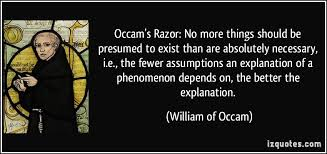
\includegraphics[width=0.99\linewidth]{occamrazor}


\end{figure}

\end{frame}
%=================================%
\begin{frame}
\begin{itemize}
\item Occam's razor (or Ockham's razor) is a principle from philosophy. Suppose there exist two explanations for an occurrence. \item In this case the simpler one is usually better. 
\item Another way of saying it is that the more assumptions you have to make, the more unlikely an explanation is. 
\item Occam's razor applies especially in the philosophy of science, but also more generally.
\end{itemize}
\end{frame}
%=================================%
\end{document}
